\section{Method}\label{sec:method}
Figure~\ref{fig:pipeline} summarises the pipeline. Given $N$ RGB views $I_1,\ldots,I_N$ from one camera translating along a row, we produce a fruit-only image in the frame of a reference view $r$. Every pixel in it is copied from a view that actually observed fruit there. The pipeline has three stages: segmentation (Sec.~\ref{sec:masks}), fruit-only registration (Sec.~\ref{sec:registration}) and observation-backed fusion (Sec.~\ref{sec:fusion}). Section~\ref{sec:evolution} explains how this design replaced an earlier depth-based prototype.

\begin{figure*}[t]
\centering
\resizebox{\textwidth}{!}{%
\begin{tikzpicture}[
  font=\footnotesize,
  >={Stealth[length=2mm]},
  box/.style={draw, rounded corners=2pt, align=center, text width=3.15cm, minimum height=1.55cm, inner sep=3pt},
  seg/.style={box, fill=green!8},
  reg/.style={box, fill=blue!7},
  fus/.style={box, fill=orange!10},
  io/.style={box, fill=gray!10},
  ev/.style={box, fill=white, dashed},
  arr/.style={->, thick},
  lab/.style={font=\scriptsize\bfseries, text=black!65}
]
% Row 1
\node[io]  (in)   {\textbf{Image sequence}\\ $N$ RGB views, one camera\\ rail (lab) or vehicle (field)};
\node[seg, right=0.55cm of in] (mask) {\textbf{Segmentation}\\ SAM~3 fruit masks $C_i$\\ foliage masks $F_i$\\ \textit{(colour rule: ablation)}};
\node[reg, right=0.55cm of mask] (sift) {\textbf{Fruit-only features}\\ SIFT on $C_i\wedge\neg F_i$\\ 4 neighbours, reciprocal\\ ratio test 0.78};
\node[reg, right=0.55cm of sift] (pair) {\textbf{Pairwise RANSAC}\\ similarity, $\tau_g{=}1.5$\,px\\ fit on $\tfrac34$, hold out $\tfrac14$\\ scale, rotation gates};
% Row 2
\node[reg, below=0.75cm of pair] (graph) {\textbf{View graph}\\ accepted pairs as edges\\ reference $r$ = best\\ connected view};
\node[reg, left=0.55cm of graph] (solve) {\textbf{Joint pose solve}\\ IRLS, $\mathcal{T}_r=\mathbf{I}$\\ drop view if held-out\\ median error $>3$\,px};
\node[fus, left=0.55cm of solve] (fuse) {\textbf{Consensus fusion}\\ warp to $r$; median colour\\ RMS $\le 30$, $\ge 3$ views\\ span $\ge 40$\,mm};
\node[io, left=0.55cm of fuse] (out) {\textbf{Fruit-only image}\\ colour copied from one\\ observing view; unseen\\ pixels left empty};
% Row 3: evaluation
\node[ev, below=0.75cm of out] (pix) {\textbf{Pixel evaluation}\\ recall, precision, IoU\\ vs.\ registered\\ leaf-free photo};
\node[ev, right=0.55cm of pix] (cnt) {\textbf{Count evaluation}\\ GrapeSAM (untuned) on\\ occluded, restored and\\ leaf-free images};
% Arrows
\draw[arr] (in) -- (mask);
\draw[arr] (mask) -- (sift);
\draw[arr] (sift) -- (pair);
\draw[arr] (pair) -- (graph);
\draw[arr] (graph) -- (solve);
\draw[arr] (solve) -- (fuse);
\draw[arr] (fuse) -- (out);
\draw[arr, dashed] (out.south) -- (pix.north);
\draw[arr, dashed] ([yshift=-0.37cm]out.south) -| (cnt.north);
\draw[arr, densely dotted] (mask.south) to[bend right=12] node[lab, pos=0.55, left] {masks} (fuse.north);
% Stage labels
\node[lab, above=1pt of mask.north] {SEGMENTATION};
\node[lab, above=1pt of sift.north east] {REGISTRATION};
\node[lab, below=1pt of pix.south east] {EVALUATION};
\node[lab, below=1pt of fuse.south east] {FUSION};
\end{tikzpicture}}
\caption{Pipeline overview. Fruit and foliage masks restrict feature matching to fruit, so that the occluding layer, which moves differently under parallax, does not drive the alignment. Pairwise similarities are combined in a view graph and solved jointly, and views failing held-out validation are dropped. Fusion keeps a pixel only when enough views, spanning enough baseline, agree on its colour, then copies that colour from one observing view. Dashed boxes are the evaluation (Sec.~\ref{sec:exp}), not part of the method.}
\label{fig:pipeline}
\end{figure*}

\subsection{Acquisition and assumptions}\label{sec:capture}
The intended field system is a side-facing smartphone on a vehicle that drives along a vine row, recording overlapping views of the canopy. To isolate the vision problem, we reproduce this motion indoors. A phone translates horizontally on a rigid rail past a scene of red grapes on branches, with removable foreground foliage in front (Fig.~\ref{fig:setup}). Illumination is held approximately constant during a sequence. The rail positions are used only to define experimental spacings and the baseline rule in Eq.~\eqref{eq:fusion}. Alignment itself is estimated from the images.

We assume that (i) the camera mainly translates parallel to the row with little rotation, (ii) the fruit layer is approximately planar, so a 2D similarity transform aligns it between nearby views, (iii) the scene is static during capture, and (iv) the foliage lies in front of the fruit, so parallax exposes different parts of the fruit in different views. Assumptions (i) and (iii) match a slow vehicle on a straight row better than handheld capture. Assumption (ii) is the weakest for deep clusters and is examined in Sec.~\ref{sec:exp}.

\begin{figure}[t]
 \centering
 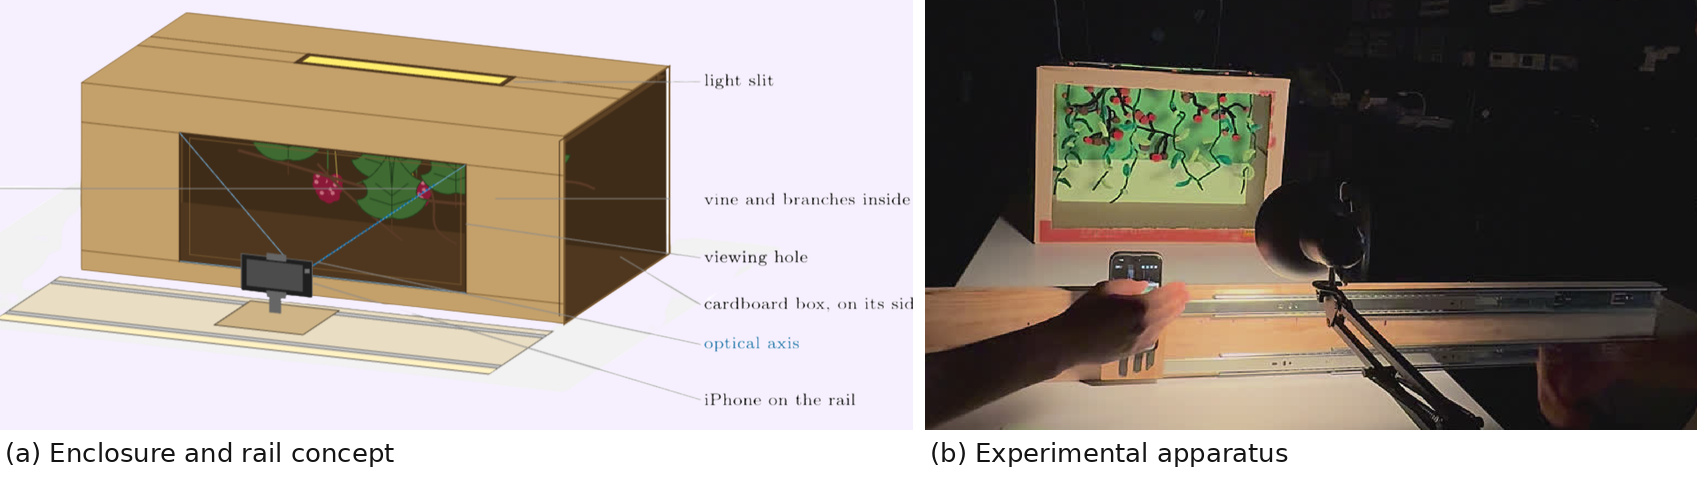
\includegraphics[width=0.86\linewidth]{figures/capture_setup.png}
 \caption{Capture rig: (a) enclosure with a horizontal camera rail and separated fruit and foliage layers, and (b) the phone, rail, lighting and scene. The rail stands in for vehicle motion along a row.}
 \label{fig:setup}
\end{figure}

\subsection{Fruit and foliage segmentation}\label{sec:masks}
For each view, we obtain a binary fruit mask $C_i(\mathbf{x})$ and a foliage mask $F_i(\mathbf{x})$ from SAM~3 text prompts~\cite{carion2025}: ``grape'' for fruit, and ``green leaf'', ``green vine'' and ``green stem'' for foliage, with fruit taking precedence where the two overlap. A pixel is usable fruit evidence when $E_i(\mathbf{x}) = C_i(\mathbf{x})\,\big(1-F_i(\mathbf{x})\big) = 1$. Excluding foliage matters at fruit boundaries, where a mask may extend over an overlapping leaf. As an ablation, we replace $C_i$ with fixed colour thresholds within a fixed region of interest. This works for red fruit against green leaves, but fails for green fruit: a green rule tuned on two captures reached only 0.31 IoU against SAM~3 masks on a held-out capture. We do not validate SAM~3's masks independently. Because the truth masks used for evaluation also come from SAM~3, the pixel-wise evaluation is not independent of this stage. On mixed red and green scenes we also split the SAM~3 fruit masks with a colour ratio rule, a qualitative step towards the ripe and unripe estimate that we do not evaluate here.

\subsection{Fruit-only registration}\label{sec:registration}
\textbf{Pairwise matching.} SIFT keypoints~\cite{lowe2004} are detected only inside the usable fruit region $E_i$. Restricting features to fruit is the key design choice. Foliage is closer to the camera and so moves further between views, and it often carries more texture, so whole-image matching would align the occluder rather than the target. Each view is matched to its next four neighbours, keeping reciprocal nearest neighbours that pass a 0.78 ratio test. A quarter of the matches are held out. A similarity transform $\mathcal{T}_{ij}$ (scale, rotation and translation) is fitted to the rest with RANSAC~\cite{fischler1981}, counting a correspondence as an inlier when
\begin{equation}
 \left\|\mathbf{p}_j - \mathcal{T}_{ij}(\mathbf{p}_i)\right\|_2 < \tau_g, \qquad \tau_g = 1.5~\text{px}.
 \label{eq:ransac}
\end{equation}
A pair is accepted only if it has at least 12 inliers and an inlier ratio of at least 0.5, if at least half of the held-out matches transfer within $2\tau_g$, and if its scale lies within 6\% of unity and its rotation within $3^\circ$. These gates follow from assumption (i). They reject pairs matched between similar-looking berries, which repeated texture makes common.

\textbf{View graph and reference.} Accepted pairs form edges of a graph over views. Only views connected to the reference can contribute. The reference is chosen automatically from the largest connected group: the view with the most accepted edges, then the most inliers, then the one closest to the group centre. If the joint solve below fails for that view, the next candidate is tried.

\textbf{Joint pose solve.} Chaining pairwise transforms accumulates drift, so we solve for one similarity $\mathcal{T}_i$ per view jointly, with $\mathcal{T}_r$ fixed to the identity:
\begin{equation}
 \min_{\{\mathcal{T}_i\}} \sum_{(i,j)\in\mathcal{E}} \sum_{k}
 w_{ijk}\,\big\|\mathcal{T}_i(\mathbf{p}^{i}_k) - \mathcal{T}_j(\mathbf{p}^{j}_k)\big\|_2^2 .
 \label{eq:joint}
\end{equation}
The problem is linear in the similarity parameters. We solve it by iteratively reweighted least squares over six iterations, with $w_{ijk}=n_{ij}^{-1}\min(1,\tau_g/e_{ijk})$. Here $e_{ijk}$ is the current residual, and $n_{ij}\le 80$ is the number of correspondences sampled from edge $(i,j)$, so that no single feature-rich pair dominates. The held-out matches are then transferred through the solved poses. Any view whose median held-out error exceeds 3~px is removed, together with its edges. A reconstruction is attempted only if at least three views remain. With SAM~3 masks at 20~mm spacing, 84--95 of 102 tested pairs passed for three to five branches, but only 40 of 98 at six branches, where 13 views were removed. More views therefore do not guarantee a larger usable aperture.

\subsection{Observation-backed fusion}\label{sec:fusion}
Each view and its masks are warped into the reference frame, $\tilde I_i(\mathbf{x}) = I_i(\mathcal{T}_i^{-1}(\mathbf{x}))$, and similarly for $\tilde E_i$. Let $\tilde V_i(\mathbf{x})$ indicate that the pixel lies inside view $i$, so that candidate observations are those with $\tilde E_i \tilde V_i = 1$. At each pixel, we take the per-channel median colour $\boldsymbol{\mu}(\mathbf{x})$ of the candidates and keep the agreeing set
\begin{equation}
 \mathcal{A}(\mathbf{x}) = \big\{\, i : \tilde E_i\tilde V_i = 1,\ d_i(\mathbf{x}) \le \tau_c \,\big\},
 \label{eq:agree}
\end{equation}
where $d_i$ is the RMS RGB distance of $\tilde I_i(\mathbf{x})$ from $\boldsymbol{\mu}(\mathbf{x})$ and $\tau_c=30$. The pixel is output as fruit when
\begin{equation}
 \hat G(\mathbf{x}) = \mathbf{1}\big[\,|\mathcal{A}(\mathbf{x})| \ge m\,\big]\;
 \mathbf{1}\big[\,B(\mathbf{x}) \ge B_{\min}\,\big],
 \label{eq:fusion}
\end{equation}
with $m=3$ views. $B(\mathbf{x})$ is the rail distance between the outermost agreeing views, and $B_{\min}=40$~mm. The median rejects a minority of misaligned or mis-segmented observations. The baseline condition requires that agreement comes from genuinely different viewpoints, not from neighbouring views that share the same occlusion.

The output colour is copied from a single agreeing view, not blended, so no colour is synthesised. The view is chosen to minimise a cost. The cost combines its smoothed colour deviation $d_i/\tau_c$, a small penalty near the boundary of its agreeing region, and a slight preference for views near the reference. This reduces visible seams between sources. Pixels with $\hat G=0$ are left empty, and fruit regions smaller than 25~px are removed. The output thus distinguishes recovered fruit from fruit that was never observed. An empty region means unobserved, not absent.

\subsection{Design evolution}\label{sec:evolution}
Our first prototype used depth-based synthetic aperture imaging~\cite{vaish2006}. For a camera translated by $B_i$ parallel to the image plane, a point at depth $Z_t$ shifts by $\Delta u_i \simeq f_x B_i / Z_t$ pixels. Shifting each view by this amount aligns the fruit plane, and the occluders, at a different depth, are blurred out by a per-pixel median or a masked mean (Fig.~\ref{fig:sai}). This required the fruit depth and the camera step to be known, and errors grow with baseline, as $\delta(\Delta u) \simeq -(f_x B_i / Z_t^2)\,\delta Z_t$. Fruit at several depths blurred, residual foliage remained, and the output was an image rather than a fruit segmentation. Replacing known geometry with fruit-only feature registration removed the need for depth and step measurements. Replacing averaging with consensus selection removed blur and produced a fruit-only output. A parallel line, a colour-free occlusion-aware synthetic aperture that finds the foliage from multi-view depth rather than colour, was developed alongside and benchmarked only on synthetic scenes; its code and results are in the repository~\cite{teamrepo}, and it is not used for the results below.

\begin{figure}[t]
 \centering
 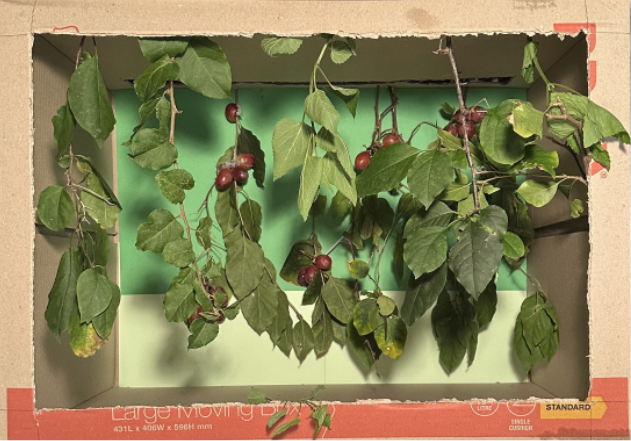
\includegraphics[width=0.44\linewidth]{figures/sai_input.png}\hfill
 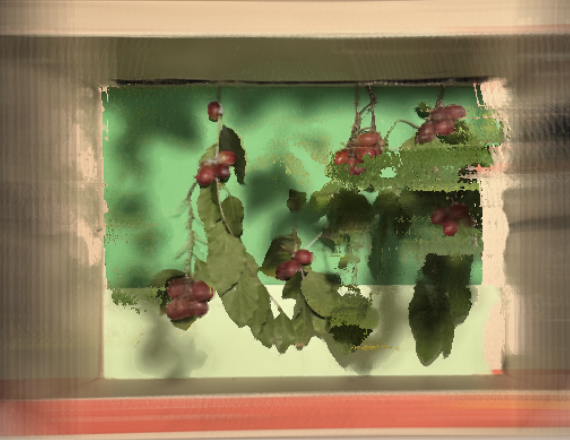
\includegraphics[width=0.44\linewidth]{figures/sai_output.png}
 \caption{Depth-based synthetic aperture prototype: occluded input (left) and fused refocused view (right). Some foliage is suppressed, but much remains, and the output is not a fruit segmentation.}
 \label{fig:sai}
\end{figure}


